%%%%%%%%%%%%%%%%%%%%%%%% INICIO QUADRO 01 %%%%%%%%%%%%%%%%%%%%%%%%%%%%%%%
\begin{table}[!ht]
  \centering
  \renewcommand{\tablename}{Quadro}
  \caption{Rudimentos de Teoria}
  \label{Quadro_01}
  \begin{tabular}[t]{|l|l|l|}
    \hline

    %%% PRÓXIMA LINHA
    \letraquadrada{A} \quadtitulo
    &
    \letraquadrada{B} \quadtitulo{Compasso}
    & 
    \letraquadrada{C} \quadtitulo{Barra de Compasso}

    

    %%% PRÓXIMA LINHA
    \\
    \begin[fragment]{lilypond}
      \transpose c c { 
        \keepWithTag #'cv
        \include "claves.ly" 
      }
    \end{lilypond}
    &
    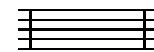
\includegraphics[scale=1]{compasso-vazio}
    &
    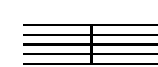
\includegraphics[scale=1]{barra-compasso}


    %%% PRÓXIMA LINHA
    \\
    \hline
    \multicolumn{2}{|l|}{\letraquadrada{D} \quadtitulo{Compasso Quaternário}}
    &    
    \letraquadrada{E} \quadtitulo{Barra Final}


    %%% PRÓXIMA LINHA
    \\
    \multicolumn{2}{|l|}{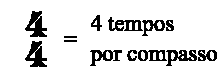
\includegraphics[scale=1]{formula-4tempos-por-compasso}}
    &
    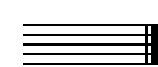
\includegraphics[scale=1]{barra-final}


    %%% FINAL DAS LINHAS
  \\
  \hline
  \end{tabular}
\end{table}    


%%%%%%%%%%%%%%%%%%%%%%%% FINAL QUADRO 01 %%%%%%%%%%%%%%%%%%%%%%%%%%%%%%%

%%% complemento do QUADRO 01
\begin{center}
%#exemplo-01#%
\end{center}


%%%%%%%%%%%%%%%%%%%%%%%% INICIO QUADRO 02 %%%%%%%%%%%%%%%%%%%%%%%%%%%%%%%
\begin{table}[!ht]
  \centering
  \renewcommand{\tablename}{Quadro}
  \caption{Cordas Soltas}
  \label{Quadro_02}
  \begin{tabular}[t]{|lll|}
    \hline


    %%% PRÓXIMA LINHA
    \letraquadrada{A} & \em & \em
   

    %%% PRÓXIMA LINHA
    \\
    \quadtitulo
    &
    \quadtitulo
    &
    \quadtitulo


    %%% PRÓXIMA LINHA
    \\
    \begin[fragment]{lilypond}
      \transpose c c {
        \keepWithTag #'cv
        \include "nota-01.ly"
      }
    \end{lilypond}
    &
    \begin[fragment]{lilypond}
      \transpose c c { 
        \keepWithTag #'cv
        \include "nota-02.ly" 
      }
    \end{lilypond}
    &
    \begin[fragment]{lilypond}
      \transpose c c { 
        \keepWithTag #'cv
        \include "nota-03.ly" 
      }
    \end{lilypond}

    \\
  \end{tabular}

  %%% PRÓXIMA TABELA
  \begin{tabular}[t]{|l|l|l|}

    %%% PRÓXIMA LINHA
    \hline
    \letraquadrada{B}  & \letraquadrada{C}   &   \letraquadrada{D}

    %%% PRÓXIMA LINHA
    \\
    \quadtitulo{Mínima}
    &
    \quadtitulo{Semínima}
    &
    \quadtitulo{Técnica}


    %%% PRÓXIMA LINHA
    \\
    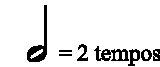
\includegraphics[scale=1]{minima}
    &
    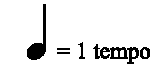
\includegraphics[scale=1]{seminima}
    &
    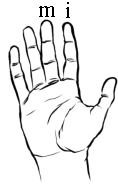
\includegraphics[scale=0.7]{mao-i-m}


    %%% PRÓXIMA LINHA
    \\
    \hline
    \letraquadrada{E}  & \letraquadrada{F} &   \letraquadrada{G}

    %%% PRÓXIMA LINHA
    \\
    \quadtitulo{Pausa de semibreve}
    &
    \quadtitulo{Pausa de mínima}
    &
    \quadtitulo{Sinal de Repetição}
    


    %%% PRÓXIMA LINHA
    \\
    
\includegraphics[scale=1]{semibreve-pausa}
    &
    
\includegraphics[scale=1]{minima-pausa}
    &
    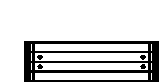
\includegraphics[scale=1]{sinal-repeticao}


    %%% FINAL DAS LINHAS
    \\
    \hline
  \end{tabular}
\end{table}    

%%%%%%%%%%%%%%%%%%%%%%%% FINAL QUADRO 02 %%%%%%%%%%%%%%%%%%%%%%%%%%%%%%%%


%%%%%%%%%%%%%%%%%%%%%%%% INICIO QUADRO 03 %%%%%%%%%%%%%%%%%%%%%%%%%%%%%%%
\begin{table}[!ht]
  \centering
  \renewcommand{\tablename}{Quadro}
  \caption{Sol Maior}
  \label{Quadro_03}
  \begin{tabular}[t]{|l|l|l|l|}
    \hline


    %%% PRÓXIMA LINHA
    \multicolumn{2}{|l|}{\letraquadrada{A}} & \multicolumn{2}{l|}{\letraquadrada{B}}
   

    %%% PRÓXIMA LINHA
    \\
    \multicolumn{1}{|l}{\quadtitulo}
    &
    \multicolumn{1}{l|}{\quadtitulo}
    &
    \multicolumn{2}{l|}{\quadtitulo{Fórmula de Compasso}}


    %%% PRÓXIMA LINHA
    \\
    \multicolumn{1}{|l}{
      \begin[fragment]{lilypond}
        \transpose c c {
          \keepWithTag #'cv
          \include "nota-04.ly"
        }
      \end{lilypond}
    }
    &
    \multicolumn{1}{l|}{
      \begin[fragment]{lilypond}
        \transpose c c {
          \keepWithTag #'cv
          \include "nota-05.ly"
        }
      \end{lilypond}
    }
    &
    \multicolumn{2}{l|}{
      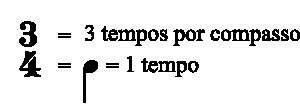
\includegraphics[scale=1]{formula-3tempos-por-compasso}
    }


    %%% PRÓXIMA LINHA
    \\
    \hline
    \letraquadrada{C} & \letraquadrada{D} & \letraquadrada{E} & \letraquadrada{F}
   

    %%% PRÓXIMA LINHA
    \\
    \quadtitulo{Sol Maior}
    &
    \quadtitulo{Andamento}
    &
    \quadtitulo{Pausa de Semínima}
    &
    \quadtitulo{Da Capo ao Fine}


    %%% PRÓXIMA LINHA
    \\
    \begin[fragment]{lilypond}
      \transpose c c {
        \keepWithTag #'cv
        \include "armadura-sol.ly"
      }
    \end{lilypond}
    &
    \textit{Allegro}
    &
    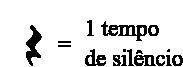
\includegraphics[scale=1]{seminima-pausa}
    &
    \textit{D.C. al Fine}


    %%% FINAL DAS LINHAS
    \\
    \hline
  \end{tabular}
\end{table}    

%%%%%%%%%%%%%%%%%%%%%%%% FINAL QUADRO 03 %%%%%%%%%%%%%%%%%%%%%%%%%%%%%%%%


%%%%%%%%%%%%%%%%%%%%%%%% INICIO QUADRO 04 %%%%%%%%%%%%%%%%%%%%%%%%%%%%%%%
\begin{table}[!ht]
  \centering
  \renewcommand{\tablename}{Quadro}
  \caption{Dlim-dlim-dlão}
  \label{Quadro_04}
  \begin{tabular}{|l|l|}
    \hline

    %%% PRÓXIMA LINHA
    \multicolumn{2}{|l|}{\letraquadrada{A}}


    %%% PRÓXIMA LINHA
    \\
    \multicolumn{1}{|l}{\quadtitulo}
    &
    \multicolumn{1}{l|}{\quadtitulo}


    %%% PRÓXIMA LINHA
    \\
    \multicolumn{1}{|l}{
      \begin{lilypond}
        \transpose c c {
          \keepWithTag #'cv
          \include "nota-06.ly"
        }
      \end{lilypond}
    }
    &
    \multicolumn{1}{l|}{
      \begin{lilypond}
        \transpose c c {
          \keepWithTag #'cv
          \include "nota-07.ly"
        }
      \end{lilypond}
    }

    %%% PRÓXIMA LINHA
    \\
    \hline
    \letraquadrada{B}   &  \letraquadrada{C}


    %%% PRÓXIMA LINHA
    \\
    \quadtitulo{Acorde}
    &
    \quadtitulo{Dinâmicas}
    

    %%% PRÓXIMA LINHA
    \\
    \begin[fragment]{lilypond}
      \transpose c c {
        \keepWithTag #'cv
        \include "acorde-G.ly"
      }
    \end{lilypond}
    &
    \textbf{\textit{f}} = forte
    

    %%% PRÓXIMA LINHA
    \\
    \em
    &
    \textbf{\textit{p}} = piano


    %%% FINAL DAS LINHAS
    \\
    \hline
  \end{tabular}
\end{table}    

%%%%%%%%%%%%%%%%%%%%%%%% FINAL QUADRO 04 %%%%%%%%%%%%%%%%%%%%%%%%%%%%%%%%



%%%%%%%%%%%%%%%%%%%%%%%% INICIO QUADRO 05 %%%%%%%%%%%%%%%%%%%%%%%%%%%%%%%
\begin{table}[!ht]
  \centering
  \renewcommand{\tablename}{Quadro}
  \caption{Lá Menor}
  \label{Quadro_05}
  \begin{tabular}{|l|l|l|}
    \hline

    %%% PRÓXIMA LINHA
    \letraquadrada{A} & \letraquadrada{B} & \letraquadrada{C}


    %%% PRÓXIMA LINHA
    \\
    \quadtitulo
    &
    \quadtitulo{Lá menor}
    &
    \quadtitulo{Fórmula de Compasso}


    %%% PRÓXIMA LINHA
    \\
    \begin{lilypond}
      \transpose c c {
        \keepWithTag #'cv
        \include "nota-08.ly"
      }
    \end{lilypond}
    &
    \begin{lilypond}
      \transpose c c {
        \keepWithTag #'cv
        \include "armadura-la-menor.ly"
      }
    \end{lilypond}
    &
    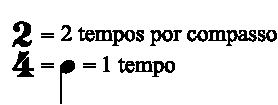
\includegraphics[scale=1]{formula-2tempos-por-compasso}
  

    %%% PRÓXIMA LINHA
    \\
    \hline
    \letraquadrada{D}  &  \letraquadrada{E}  &  \letraquadrada{F}


    %%% PRÓXIMA LINHA
    \\
    \quadtitulo{Andamento}
    &
    \quadtitulo{Crescendo}
    &
    \quadtitulo{Decrescendo}

    %%% PRÓXIMA LINHA
    \\
    \textit{Andante}
    &
    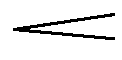
\includegraphics[scale=1]{crescendo}
    &
    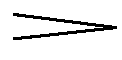
\includegraphics[scale=1]{decrescendo}

    \\
  \end{tabular}

  %%% PRÓXIMA TABELA
  \begin{tabular}[t]{|llll|}

    %%% PRÓXIMA LINHA
    \hline
    \multicolumn{4}{|l|}{\letraquadrada{G}}
    
    %%% PRÓXIMA LINHA
    \\
    \multicolumn{4}{|l|}{\quadtitulo{Acordes}}

    
    %%% PRÓXIMA LINHA
    \\
    \begin[fragment]{lilypond}
      \transpose c c { 
        \keepWithTag #'cv
        \include "acorde-D.ly"
      }
    \end{lilypond}
    &
    \begin[fragment]{lilypond}
      \transpose c c { 
        \keepWithTag #'cv
        \include "acorde-D7.ly" 
      }
    \end{lilypond}
    &
    \begin[fragment]{lilypond}
      \transpose c c {
        \keepWithTag #'cv
        \include "acorde-Am.ly"
      }
    \end{lilypond}
    &
    \begin[fragment]{lilypond}
      \transpose c c {
        \keepWithTag #'cv
        \include "acorde-E7.ly"
      }
    \end{lilypond}


    %%% FINAL DAS LINHAS
    \\
    \hline
  \end{tabular}
\end{table}    

%%%%%%%%%%%%%%%%%%%%%%%% FINAL QUADRO 05 %%%%%%%%%%%%%%%%%%%%%%%%%%%%%%%%



%%%%%%%%%%%%%%%%%%%%%%%% INICIO QUADRO 06 %%%%%%%%%%%%%%%%%%%%%%%%%%%%%%%
\begin{table}[!ht]
  \centering
  \renewcommand{\tablename}{Quadro}
  \caption{A Margarida}
  \label{Quadro_06}
  \begin{tabular}{|l|l|}
    \hline

    %%% PRÓXIMA LINHA
    \letraquadrada{A} & \letraquadrada{B}


    %%% PRÓXIMA LINHA
    \\
    \quadtitulo
    &
    \quadtitulo{Colcheias}


    %%% PRÓXIMA LINHA
    \\
    \begin{lilypond}
      \transpose c c {
        \keepWithTag #'cv
        \include "nota-09.ly"
      }
    \end{lilypond}
    &
    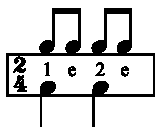
\includegraphics[scale=1]{duas-colcheias}


    %%% PRÓXIMA LINHA
    \\
    \hline
    \letraquadrada{C}  &  \letraquadrada{D}


    %%% PRÓXIMA LINHA
    \\
    \quadtitulo{Ligadura de Frase}
    &
    \quadtitulo{Anacruse}


    %%% PRÓXIMA LINHA
    \\
    
\includegraphics[scale=1]{ligadura-frase}
    &
    \parbox[b][1cm]{9cm}{
      Note que a lição \textit{``\nameref{sec:impr-em-margarida}''} na
      página \pageref{sec:impr-em-margarida} começa no 4º
      tempo do compasso.
    }

    %%% FINAL DAS LINHAS
    \\
    \hline
  \end{tabular}
\end{table}    

%%%%%%%%%%%%%%%%%%%%%%%% FINAL QUADRO 06 %%%%%%%%%%%%%%%%%%%%%%%%%%%%%%%%


%%%%%%%%%%%%%%%%%%%%%%%% INICIO QUADRO 07 %%%%%%%%%%%%%%%%%%%%%%%%%%%%%%%
\begin{table}[!ht]
  \centering
  \renewcommand{\tablename}{Quadro}
  \caption{Dó Maior}
  \label{Quadro_07}
  \begin{tabular}{|ll|l|l|}
    \hline

    %%% PRÓXIMA LINHA
    \multicolumn{2}{|l|}{\letraquadrada{A}} & \letraquadrada{B} & \letraquadrada{C}


    %%% PRÓXIMA LINHA
    \\
    \quadtitulo
    &
    \quadtitulo
    &
    \quadtitulo{Andamento}
    &
    \quadtitulo{Dinâmica}


    %%% PRÓXIMA LINHA
    \\
    \begin{lilypond}
      \transpose c c {
        \keepWithTag #'cv
        \include "nota-10.ly"
      }
    \end{lilypond}
    &
    \begin{lilypond}
      \transpose c c {
        \keepWithTag #'cv
        \include "nota-11.ly"
      }
    \end{lilypond}
    &
    \textit{Moderado}
    &
    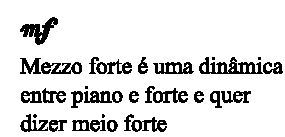
\includegraphics[scale=1]{mezzo-forte}


    %%% PRÓXIMA LINHA
    \\
    \hline
    \multicolumn{2}{|l|}{\letraquadrada{D}}  &  \multicolumn{2}{l|}{\letraquadrada{E}}


    %%% PRÓXIMA LINHA
    \\
    \multicolumn{2}{|l|}{\quadtitulo{Acordes}}
    &
    \multicolumn{2}{l|}{\quadtitulo{Pausa de Compasso}}


    %%% PRÓXIMA LINHA
    \\
    \multicolumn{1}{|l}{
      \begin{lilypond}
        \transpose c c {
          \keepWithTag #'cv
          \include "acorde-C.ly"
        }
      \end{lilypond}
    }
    &
    \multicolumn{1}{l|}{
      \begin{lilypond}
        \transpose c c {
          \keepWithTag #'cv
          \include "acorde-G7.ly"
        }
      \end{lilypond}
    }
    &
    \multicolumn{2}{c|}{
      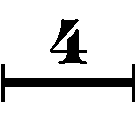
\includegraphics[scale=.7]{4compassos-pausa}
    }

    %%% PRÓXIMA LINHA
    \\
    \multicolumn{2}{|l|}{
      \em
    }
    &
    \multicolumn{2}{l|}{
      \parbox[b][1cm]{9cm}{
        Note que na lição \textit{``\nameref{sec:marcha-soldado}''} na
        página \pageref{sec:marcha-soldado} há indicação de 4 compassos
        em pausa.
      }
    }

    %%% FINAL DAS LINHAS
    \\
    \hline
  \end{tabular}
\end{table}    

%%%%%%%%%%%%%%%%%%%%%%%% FINAL QUADRO 07 %%%%%%%%%%%%%%%%%%%%%%%%%%%%%%%%



%%%%%%%%%%%%%%%%%%%%%%%% INICIO QUADRO 08 %%%%%%%%%%%%%%%%%%%%%%%%%%%%%%%
\begin{table}[!ht]
  \centering
  \renewcommand{\tablename}{Quadro}
  \caption{Sol Mixolídio}
  \label{Quadro_08}
  \begin{tabular}{|l|l|}
    \hline

    %%% PRÓXIMA LINHA
    \multicolumn{2}{|l|}{\letraquadrada{A}}


    %%% PRÓXIMA LINHA
    \\
    \multicolumn{1}{|l}{
      \quadtitulo
    }
    &
    \multicolumn{1}{l|}{
      \quadtitulo
    }

    %%% PRÓXIMA LINHA
    \\
    \multicolumn{1}{|l}{
      \begin{lilypond}
        \transpose c c {
          \keepWithTag #'cv
          \include "nota-12.ly"
        }
      \end{lilypond}
    }
    &
    \multicolumn{1}{l|}{
      \begin{lilypond}
        \transpose c c {
          \keepWithTag #'cv
          \include "nota-13.ly"
        }
      \end{lilypond}
    }

    %%% PRÓXIMA LINHA
    \\
    \hline
    \letraquadrada{B}  &  \letraquadrada{C}


    %%% PRÓXIMA LINHA
    \\
    \quadtitulo{Fermata}
    &
    \quadtitulo{Andamento}


    %%% PRÓXIMA LINHA
    \\
    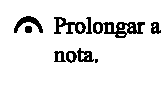
\includegraphics[scale=1]{fermata}
    &
    \textit{Adagio}


    %%% FINAL DAS LINHAS
    \\
    \hline
  \end{tabular}
\end{table}    

%%%%%%%%%%%%%%%%%%%%%%%% FINAL QUADRO 08 %%%%%%%%%%%%%%%%%%%%%%%%%%%%%%%%


%%%%%%%%%%%%%%%%%%%%%%%% INICIO QUADRO 09 %%%%%%%%%%%%%%%%%%%%%%%%%%%%%%%
\begin{table}[!ht]
  \centering
  \renewcommand{\tablename}{Quadro}
  \caption{Transposição}
  \label{Quadro_09}
  \begin{tabular}{|l|l|}
    \hline

    %%% PRÓXIMA LINHA
    \letraquadrada{A} & \letraquadrada{B}


    %%% PRÓXIMA LINHA
    \\
    \quadtitulo{Semínima Pontuada}
    &
    \quadtitulo{Pausa de Colcheia}
    

    %%% PRÓXIMA LINHA
    \\
    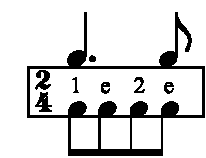
\includegraphics[scale=1]{seminima-pontuada}
    &
    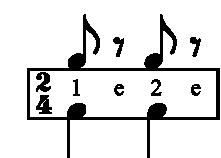
\includegraphics[scale=1]{colcheia-pausa}

    %%% PRÓXIMA LINHA
    \\
    \hline
    \letraquadrada{C}  &  \letraquadrada{D}


    %%% PRÓXIMA LINHA
    \\
    \quadtitulo{Dinâmica}
    &
    \quadtitulo{Ligadura de Prolongamento}


    %%% PRÓXIMA LINHA
    \\
    \textit{cresc.} = crescendo
    &
    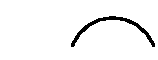
\includegraphics[scale=1]{ligadura-prolongamento}


    %%% PRÓXIMA LINHA
    \\
    \textit{decresc.} = decrescendo
    &
    \em


    %%% FINAL DAS LINHAS
    \\
    \hline
  \end{tabular}
\end{table}    

%%%%%%%%%%%%%%%%%%%%%%%% FINAL QUADRO 09 %%%%%%%%%%%%%%%%%%%%%%%%%%%%%%%%



%%%%%%%%%%%%%%%%%%%%%%%% INICIO QUADRO 10 %%%%%%%%%%%%%%%%%%%%%%%%%%%%%%%
\begin{table}[!ht]
  \centering
  \renewcommand{\tablename}{Quadro}
  \caption{Síncopa}
  \label{Quadro_10}
  \begin{tabular}{|ll|l|l|}
    \hline

    %%% PRÓXIMA LINHA
    \multicolumn{2}{|l|}{\letraquadrada{A}} & \letraquadrada{B} & \letraquadrada{C} 


    %%% PRÓXIMA LINHA
    \\
    \multicolumn{1}{|l}{
      \quadtitulo
    }
    &
    \multicolumn{1}{l|}{
      \quadtitulo
    }
    &
    \quadtitulo{Mínima Pontuada}
    &
    \quadtitulo{Síncopa}


    %%% PRÓXIMA LINHA
    \\
    \multicolumn{1}{|l}{
      \begin{lilypond}
        \transpose c c {
          \keepWithTag #'cv
          \include "nota-14.ly"
        }
      \end{lilypond}
    }
    &
    \multicolumn{1}{l|}{
      \begin{lilypond}
        \transpose c c {
          \keepWithTag #'cv
          \include "nota-15.ly"
        }
      \end{lilypond}
    }
    &
    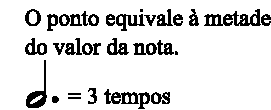
\includegraphics[scale=1]{minima-pontuada}
    &
    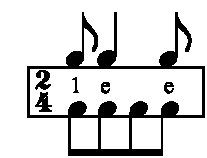
\includegraphics[scale=1]{ritmo-848}


    %%% PRÓXIMA LINHA
    \\
    \hline
    \multicolumn{2}{|l|}{\letraquadrada{D}} & \letraquadrada{E} & \letraquadrada{F} 

    %%% PRÓXIMA LINHA
    \\
    \multicolumn{2}{|l|}{
      \quadtitulo{Primera e Segunda Vez}
    }
    &
    \quadtitulo{Sustenido}
    &
    \quadtitulo{Bequadros}


    %%% PRÓXIMA LINHA
    \\
    \multicolumn{2}{|l|}{
      \includegraphics[scale=1]
    }
    &
    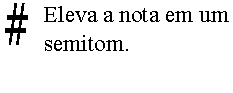
\includegraphics[scale=1]{sustenido}
    &
    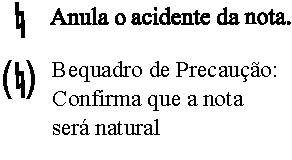
\includegraphics[scale=1]{bequadro-pre}



    %%% FINAL DAS LINHAS
    \\
    \hline
  \end{tabular}
\end{table}    

%%%%%%%%%%%%%%%%%%%%%%%% FINAL QUADRO 10 %%%%%%%%%%%%%%%%%%%%%%%%%%%%%%%%
















